\documentclass[Main.tex]{PositionOgSkalering}

\begin{document}
\chapter{Position og skalering}
Hvis man lave et  2d spil uden et moderne framework eller engine, ligner det en nem løsning at basere sit spil på skærm koordinator. Vi har et eksempel på dette type system fra et forrigt projekt kaldet MAD \ref{MADscaling1}, og har ud fra det og andre projekter lært hvad problemet ved skærm koordinater, også kaldt pixel koordinater, er, hvilket for det meste hænger sammen med skærmopløsningen.

\begin{figure}[h]
\centering
\parbox{7cm}{   
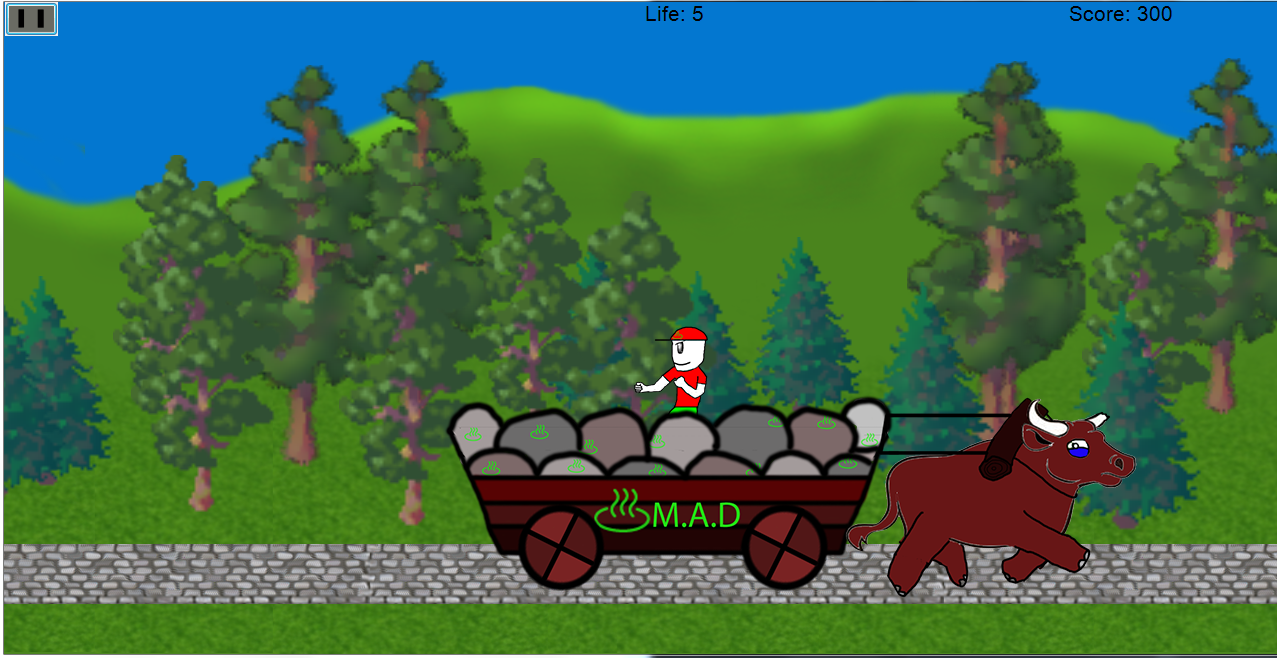
\includegraphics[width = 7cm]{billeder/MADscaling1}
\caption{MAD i produktions opløsning}    
\label{MADscaling1}}
\qquad
\begin{minipage}{7cm}
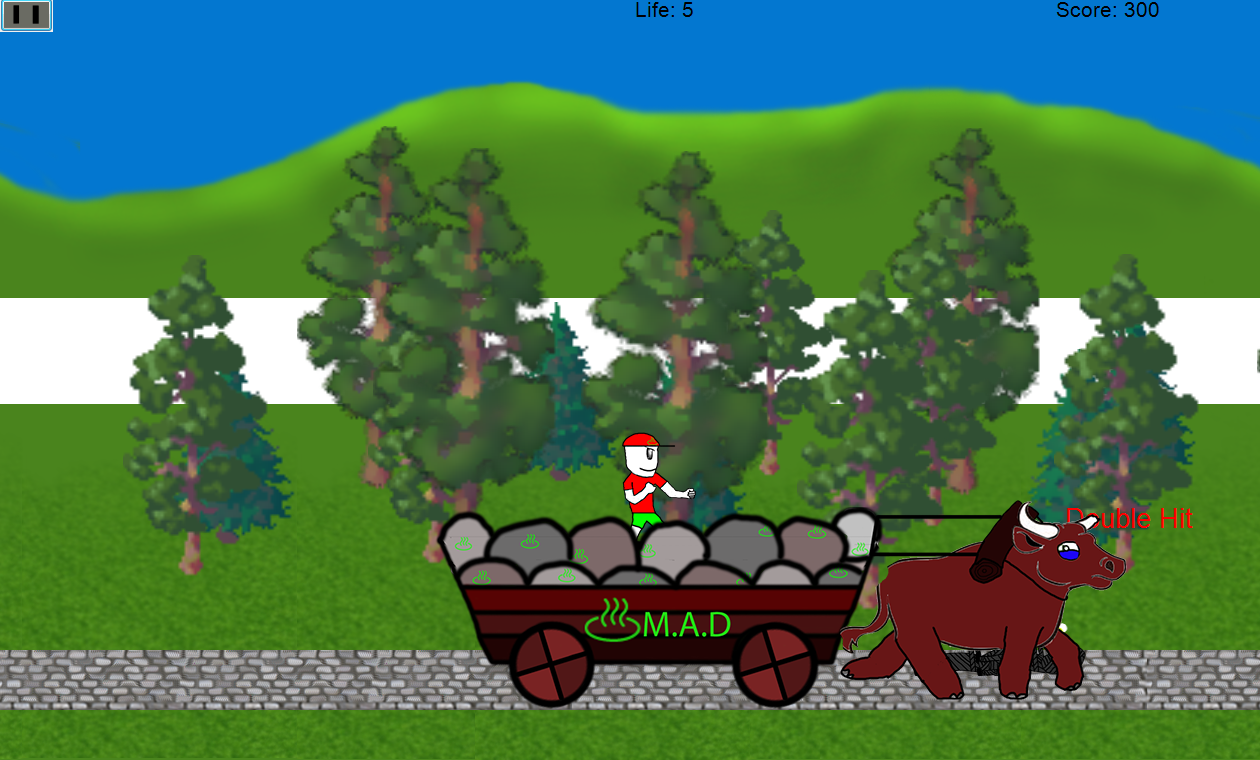
\includegraphics[width = 7cm]{billeder/MADscaling2}
\caption{MAD i 1280x800 opløsning med skærm kordinator}    
\label{MADscaling2}
\end{minipage}
\end{figure}

Problemerne ved et skærm koordinatsystem opstår når skærmstørrelsen bliver ændret. Eks. hvis man vil have et objekt nede i det højre hjørne af skærmen, kan der ske problemer når  skærmopløsningen ændres, På figur \ref{MADscaling1} og \ref{MADscaling2} kan man se to forskellige opløsninger. På figur \ref{MADscaling1} er det nederste højre hjørne koordinatet 1290,690, og på det figur \ref{MADscaling2} er det 1280,800. Fordi det ene spil er 110 pixel højere end det originale, betyder det at der er 110 pixels ned af y-aksen, som programmet ikke bruger.

Hvis man så også skal skalerer alle spilobjekterne så de passer bedre til den nye opløsning, skal de skaleres med ca. 16\% \begin{math} (110 \div 690  = 0.1594203 \approx 0.16) \end{math}på y-aksen. Udover at det kommer til at se mærkeligt ud når spilobjekterne bliver skaleret, passer deres nye størrelse ikke til deres placering. Dette kan bedre ses på figur \ref{MADscaling4}, hvor opløsningen er 860x345. Dette forårsage at man ikke kan se andet end baggrunden, fordi alle objekterne starter i højere koordinater end hvad skærmen indeholder.

\begin{figure}[h]
\centering
\parbox{7cm}{   
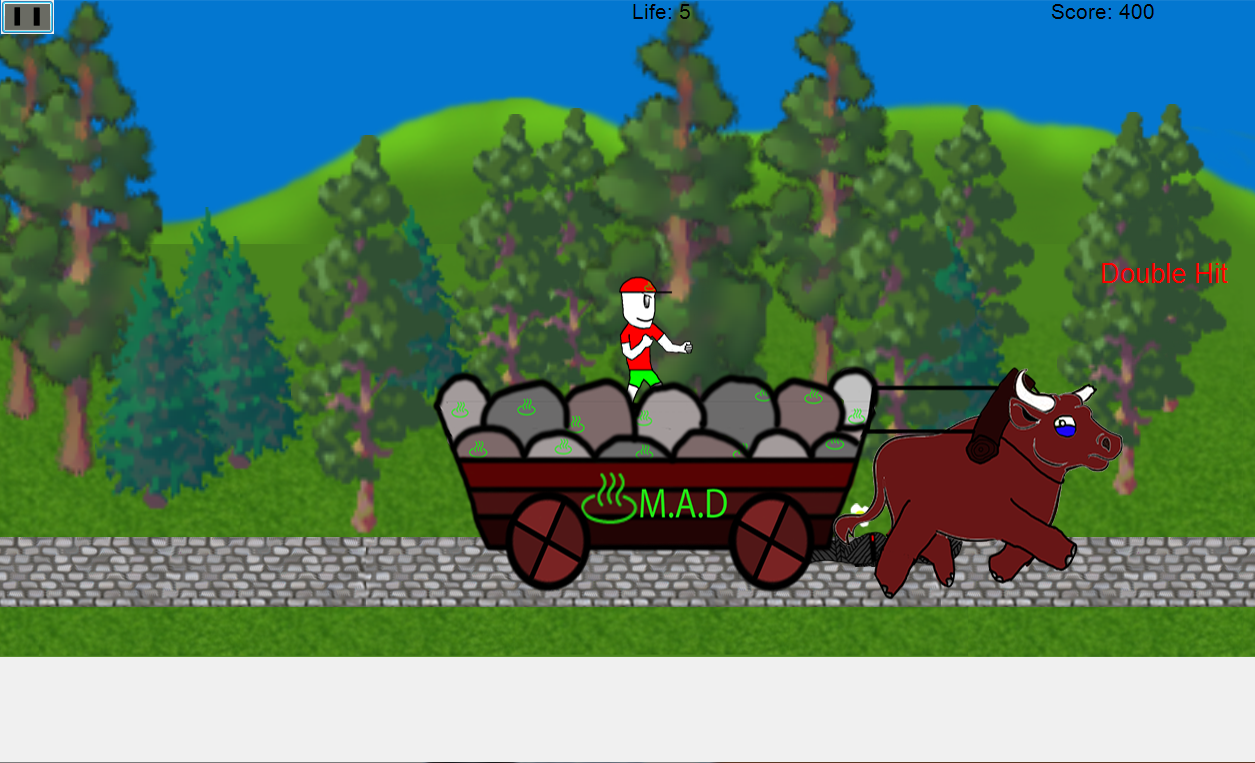
\includegraphics[width = 7cm]{billeder/MADscaling3}
\caption{MAD hvor alle sprites er skaleret 16\% på y aksen}    
\label{MADscaling3}}
\qquad
\begin{minipage}{7cm}
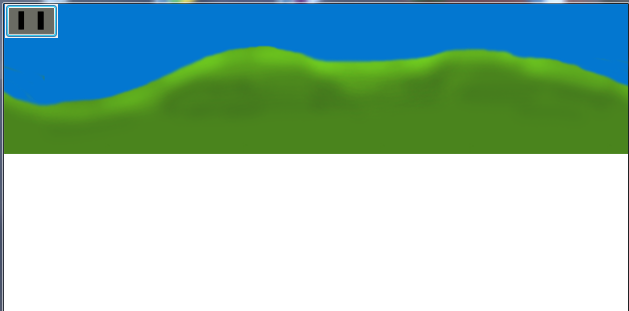
\includegraphics[width = 7cm]{billeder/MADscaling4}
\caption{MAD i opløsningen 860x345}    
\label{MADscaling4}
\end{minipage}
\end{figure}

Et andet problem kan være spil objekternes kollisionsboks, da deres størrelse også kan være i pixels. Hvis et spilobjekts sprite nedskaleres uden at dets kollisions boks skaleres, vil objektets visuelle repræsentation være ude af sync med dets faktiske position og størrelse. Se figur \ref{MADscaling5} fra MAD, hvor positionen følger med opløsningen, men nogle af kollisionsboksene ikke gør, især vognens kollisionsboks. 

\begin{figure}[h]
\centering
\parbox{7cm}{   
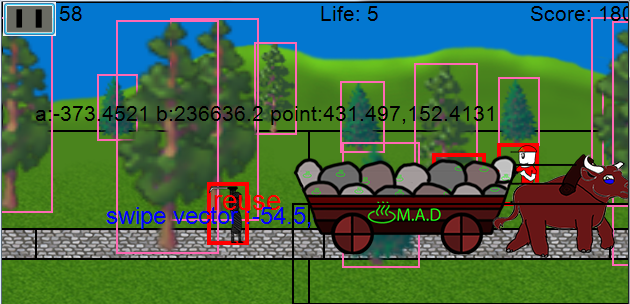
\includegraphics[width = 7cm]{billeder/MADscaling5}
\caption{MAD hvor kollisionsboksene ikke er relative til spilobjekternes størrelse}    
\label{MADscaling5}}
\qquad
\begin{minipage}{7cm}
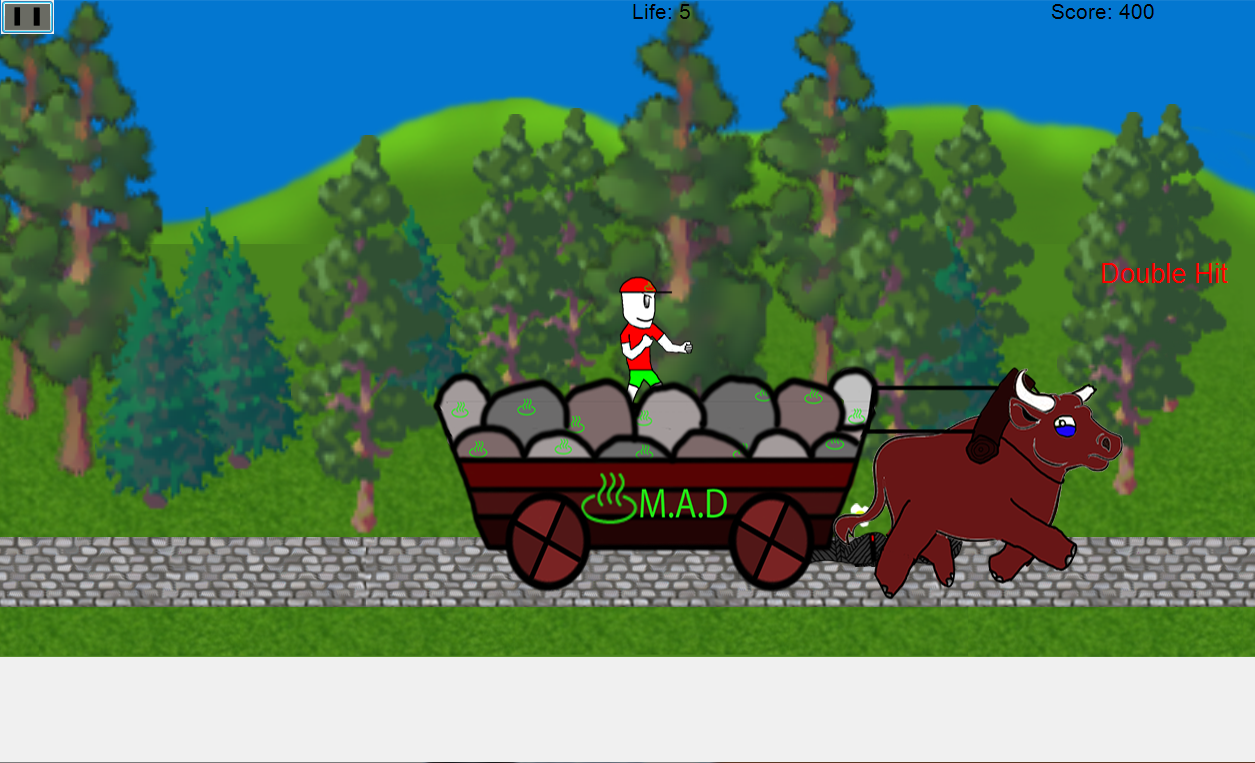
\includegraphics[width = 7cm]{billeder/MADscaling6}
\caption{MAD hvor kollisionsboksene er relative til spilobjekternes størrelse}    
\label{MADscaling6}
\end{minipage}
\end{figure}

En løsning vi fandt til disse problemer, er ved at lave koordinaterne i forhold til skærmopløsning. metoden for dette kunne være: \\*\\*
\begin{math}
\text{Produktions X } \times (\text{faktisk skærmbredde} \div \text{produktions skærmbredde}), \\*
\text{Produktions Y} \times (\text{faktisk skærmhøjde} \div \text{productions skærmhøjde})\end{math} \\* \\*
Det sammen kan gøres med kollisions boksen, bare hvor det er i forhold til spriten:\\*\\*
\begin{math}\text{Produktions kollisions boks bredde} \times (\text{faktisk spritebredde} \div \text{Produktions spritebredde}),\\*
\text{produktions kollisions boks højde} \times (\text{faktisk spritehøjde} \div \text{produktions spritehøjde}).  \end{math}\\*

Disse udregninger er brugt I MAD, se figur \ref{MADscaling6}, hvilket har løst problemerne involveret med fejlplaceret objekter og kollisionbokse.
En anden løsning er at unlade at kode i skærm koordinator, og have game world koordinator, som ved hjælp af en kamera klasse, kan konverteres til skærm koordinator. Se bilaget for et eksempel af en kamera klasse skrevet i C\#.
Mange moderne frameworks og engines bruger også spilverdenens koordinater, eksempelvis Unity \cite{unity3d}.

\section{Tekstur skalering}
I konstruktionen af assets til spil, er det et krav at teksturer og sprites skal kunne skalere efter skærmopløsningen på en given platform. En umiddelbar løsning ville indebære at tegne alle visuelle assets i høj opløsning og dermed sikrer at en høj kvalitet bliver opnået på høje skærmopløsninger \cite{deepworldgame}.

Der opstår dog problemer når man skalerer ned. Hvis man f.eks. skalerer fire pixels ned til det halve, får man to pixels, men skalere man tre pixels ned til det halve, får man 1,5 pixels. Da man ikke kan have halve pixels, et det enten én eller to pixels man ender op med, hvilket kan få grafikken til at se aliased ud \cite{Martin}. Mange moderne algoritmer prøver selv at løse problemet så det er mindre tydeligt at teksturen er blevet skaleret.\cite{Kopf} Det kan dog stadig være synligt, og desuden tager det også længere tid at lave en teksture med meget høj opløsning, end et med lavere opløsning. En anden løsning  kunne lave er at lave teksturene med lav opløsning, og derefter skalere dem op. Dette får dog teksturene til at se pixelerede ud \cite{McHugh}.

En tredje måde at gøre det på er at lave vektorgrafik, da de skalerer uendligt \cite{deepworldgame}. Det tager dog længere tid at lave vektorgrafik end normal grafik,\cite{deepworldgame} og derudover kræver vektorgrafik også mere cpu kraft, men mindre ram \cite{deepworldgame}. Derfor er der nogle platforme hvorpå vektorgrafik kan funkere bedre end andre, da cpu varierer meget fra platform til platform \cite{PassMark}.

Der er ikke en bedste måde at løse skaleringsproblemer på, da det afhænger meget af det spil man laver, og hvor lang tid man har til at lave det. Generelt er det en god idé at lave teksturer i høj opløsning, da meget morderen software sørger for at det stadig ser godt ud når det bliver nedskaleret.
\end{document}

\begin{figure}[p]
\lstset{numbers=left, language=[Sharp]C}
\lstinputlisting[caption = Et eksempel på en kamera klasse, label = kameraKlasse]{kode/Kamera.cs}
\end{figure}
